%\documentclass[12pt]{scrreprt}
\documentclass[12pt]{report}

% language may be romanian or english (default is english)
% type may be bachelor or master (default is bachelor)
\usepackage[language=english, type=bachelor]{style}

%\geometry{a4paper,top=2.5cm,left=3cm,right=2.5cm,bottom=2.5cm}
%in style
%controlling the appearance of your headers and footers
\usepackage{fancyhdr}
\pagestyle{fancy}
\lhead{}
\chead{}
\renewcommand{\headrulewidth}{0.2pt}
\renewcommand{\footrulewidth}{0.2pt}

\begin{document}

\specialization{COMPUTER SCIENCE}
\title{Using artificial intelligence to assist chess players}
\author{Cadar Eduard}
\supervisor{Asist. univ. dr. Florentin Bota}
\maketitle

\specialization{INFORMATICĂ}
\title{Utilizarea inteligenței artificiale în asistarea jucătorilor de șah}
\author{Cadar Eduard}
\supervisor{Asist. univ. dr. Florentin Bota}
\maketitle

\newpage
\thispagestyle{empty}
\mbox{}
\newpage
\pagenumbering{roman} 

\cleardoublepage
ABSTRACT
\vspace{0.5cm}	
\hrule
\vspace{0.5cm}	
%\cleardoublepage

The usual way of searching for a move from a chess position is through tactics or strategy. Tactics are series of moves that would bring an immediate advantage, while strategy refers to a general 'sense' of advantage on the board (having better developed pieces, better pawn structure etc.).

Chess engines are usually built using a minimax algorithm. This approach is able to find the moves that would bring material gain (capturing pieces) in a given depth, but cannot find moves that would slowly improve the position. A neural network trained on professional chess games is able to find good positional moves, but may be weak at finding tactical moves.

An algorithm combining these two approaches should yield better results than each of them on their own.

Abstract: un rezumat \^{i}n limba englez\u{a} cu prezentarea, pe scurt, a con\c{t}inutului pe capitole, pun\^{a}nd accent pe contribu\c{t}iile proprii \c{s}i originalitate

\tableofcontents

\newpage
\pagenumbering{arabic}

\chapter{Introduction}
% \chapter*{Introducere}
\label{intro}

% Introducere: obiectivele lucrarii si descrierea succinta a capitolelor, prezentarea temei, prezentarea contributiei proprii, respectiv a rezultatelor originale

Despite being a centuries-old game, chess still remains unsolved, and is one of the most extensively researched areas of artificial intelligence. Due to the complexity of the game and the large number of possible positions, conventional methods of computing and searching for the best move are ineffective and produce unsatisfactory results, necessitating the use of heuristics in search, evaluation, and move selection.

Chess needs so much creativity and profound reasoning that it was originally considered that computers would never be able to perform it. And it remained that way for a long time, until IBM's Deep Blue \cite{campbell2002deep} defeated reigning World Chess Champion Garry Kasparov in 1997, winning 2 matches, drawing 3, and losing 1. Since then, the best chess engines have improved to the point that no human is able to win a single match against them.

% Chess engines operate ... different than humans - humans look into less branches (are more selective), while engines brute-force almost all the branches

There are several properties of the chess game that make it ideal for computers:
\begin{itemize}
    \item Deterministic - all potential games result in either a win for white, a draw, or a win for black
    \item Finite - games cannot continue indefinitely (there are two restrictions to avoid this: a draw occurs after three repetitions of the same position, and 50 moves without a capture or a pawn move is also a draw)
    \item Complete information - there is no concealed information or ambiguity as there is in a card game, and the game is played sequentially; both players have access to the same information
    \item Zero-sum - the goals of the competitors are opposite: a win for one player is a loss for his opponent, and a draw results in a game sum of zero. If a position is worth +10 to one player, then the opponent's score is -10
\end{itemize}

In the next chapter some of the techniques and algorithms used in programming chess engines are described, as well as some of the optimization methods that modern chess engines utilize. In the third chapter an introduction is given to the state of the art in chess engines and how an engine's strength is determined. In the fourth chapter I will describe the methods and algorithms I used in building my chess engine, and in the fifth chapter I will describe the tools and technologies with which I built the game and the engine. The sixth chapter presents an evaluation of the engine, and in the seventh chapter the conclusions of the work are highlighted.
%\addcontentsline{toc}{chapter}{Introducere}
%\addcontentsline{toc}{chapter}{Introduction}

\chapter{Background}
\label{chap:ch2}

\indent\par Informatii si citare carte \cite{Sommerville2010}.

\section{Methods used}
\label{sec:ch2sec1}

\par Methods/algorithms used in programming and training chess engines.

\section{State of the art chess engines}
\label{sec:ch2sec2}

\par Stockfish, AlphaZero etc. - overview and AI techniques used in them 

% Informatii si citare articol publicat la conferinta (in proceedings) \cite{Narayan2012}.

% Informatii si citare articol publicat în revista \cite{Robbes2015}.

% Informatii si citare articol publicat tip masterthesis  \cite{mastersthesis1993}.

% Informatii si citare articol publicat tip phdthesis \cite{phdthesis1993}.

% Informatii si citare articol ca resursa Internet  \cite{kinaSUR}.

% Inserarea si Referirea unei figuri \ref{FigCBSD}.

% \begin{figure}[htbp]
% 	\centering
% 		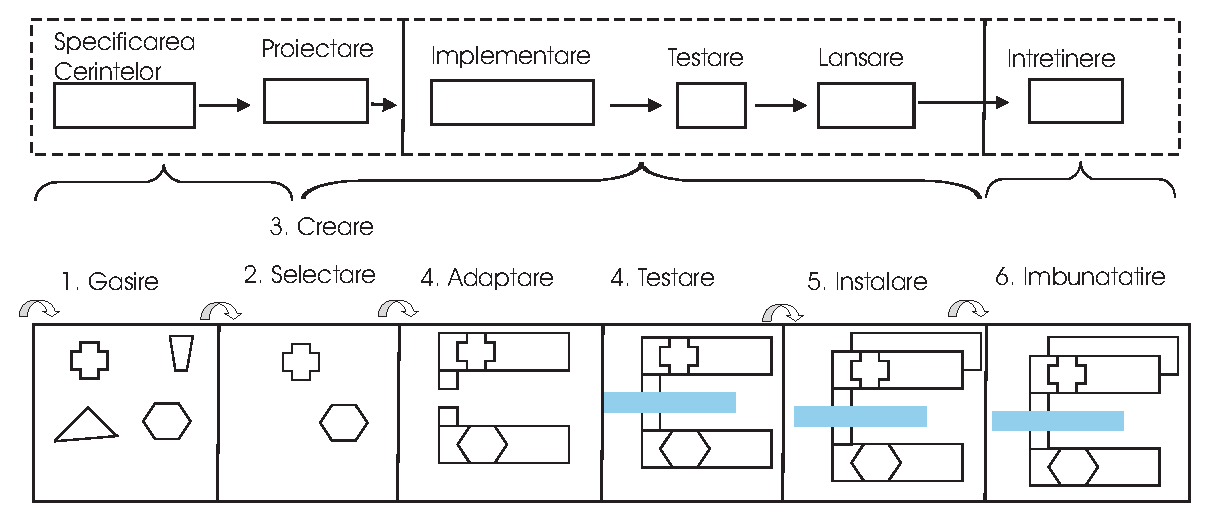
\includegraphics[scale=0.65]{./figures/fig_3_1.eps}
% 	\caption{Ciclul de dezvoltare al sistemelor bazate pe componente adaptat modelului cascadã}
% 	\label{FigCBSD}
% \end{figure}

% Inserarea si Referirea la Tabelul \ref{TabelSolutii}.

% \begin{table}[htbp]
% \begin{center}
% \begin{tabular}
% {|p{120pt}|p{120pt}|p{120pt}|}
% \hline
%  Nume algoritm  &  Toate solutiile &  Solutia optimã\\
% \hline 
% \hline Nume 1 & $20$ & $5$  \\
% \hline Nume 2 & $20$ & $2$  \\
% \hline
% \end{tabular}
% \end{center}
% \caption{Solutii obtinute }
% \label{TabelSolutii}
% \end{table}

% Adaugarea si Referirea la o Ecuatie \ref{LabelMyEquation}.

%  \begin{equation}
%      ws_N4 = w_{14}*N1 + W_{24}+N2 + w_{34}*N3
% \label{LabelMyEquation}
%  \end{equation}
 

\chapter{State of the art chess engines}
\label{chap:ch3}

\section{Top Chess Engine Championship}
\label{sec:ch3sec1}

The Top Chess Engine Championship (TCEC) is internationally recognized as one of the most prestigious and competitive computer chess tournaments in the world.

TCEC is an online tournament that features the strongest chess engines competing in a round-robin format (each engine plays in turn against every other engine), followed by knockout stages to determine the champion. The engines compete on powerful hardware, and each match consists of multiple games with different time controls and openings to ensure a diverse range of positions and scenarios.

TCEC has been held several times a year since 2010, and 24 seasons have concluded as of May 2023. Stockfish holds the record of being a 14-time winner of the TCEC. Stockfish and Leela Chess Zero have dominated the competition in the past years, with the final having been played between the two engines in 9 of the last 11 seasons.

\section{Elo rating system}
\label{sec:ch3sec2}

The Elo rating system is a technique used to determine the comparative levels of skill among players in games with zero-sum outcomes. FIDE (Fédération Internationale des Échecs), the international governing body for chess, embraced the Elo rating system in 1970 and continues to employ it as the primary method for evaluating player skill to this present day.

A player's Elo rating is denoted by a numerical value that might increase or decrease based on the outcomes of the rated games they play.

Elo's rating system operates on the premise that every player possesses an unknown current playing ability, which is approximated by a rating. When players with (unknown) strengths $R_A$ and $R_B$ engage in a game, the projected score for player A is assumed to be

\begin{equation}
    E=\frac{1}{1+10^{-(R_A-R_B)/400}},
\end{equation}

where the score corresponds to 1 in the event of player A's victory, $1/2$ in case of a draw, and 0 if player A loses \cite{glickman1999rating}.

Following each match, the victorious player subtracts rating points from their defeated opponent, with the total points gained or lost being determined by the disparity in their ratings. If the player with a higher rating wins, only a small number of rating points are deducted from the lower-rated player. Conversely, if the lower-rated player achieves an unexpected victory, a substantial number of rating points is transferred from the higher-rated player to the lower-rated player.

When a game results in a draw, the lower-rated player receives a small number of points from the higher-rated player. Therefore, this rating system possesses a self-correcting mechanism. Players whose ratings are either too low or too high will eventually outperform or underperform, respectively, compared to the expectations set by the rating system. Consequently, these players will gain or lose rating points until their ratings align with their true playing ability.

Elo ratings are solely comparative and hold validity only within the specific rating pool in which they were computed, rather than serving as an absolute measure of a player's proficiency. The highest Elo rating attained by a human was 2882, accomplished by Magnus Carlsen in May 2014 on the FIDE ratings list \cite{fide-ratings-May2014}. It is estimated that top chess engines possess over 3400 Elo points.

\section{Stockfish}
\label{sec:ch3sec3}

The strongest chess engine is currently Stockfish, an open-source project. It uses a minimax algorithm to search for the most promising positions, along with alpha-beta pruning, iterative deepening, and other improvements to reduce the search-space \cite{maharaj2022chess}. For evaluating the positions, Stockfish uses a hand-crafted evaluation function that consists of multiple features: material, position of the pieces on the board, structure of the pawns, mobility of pieces, safety of the king etc. \cite{lai2015giraffe}

Recent versions of Stockfish have been improved with NNUE (Efficiently Updatable Neural Networks). NNUE is a neural network-based evaluation function. Unlike traditional evaluation functions that are based on handcrafted features and heuristics, NNUE evaluates a chess position by analyzing it directly with a neural network. Because the neural network can learn and improve its evaluation of positions over time through training, the evaluation function becomes more flexible and adaptable.

Stockfish uses a multi-layer neural network architecture that receives a representation of the present board state as input and generates a score that reflects the anticipated outcome of the game. The neural network is trained using a dataset of high-quality chess games, where the inputs are positions from the games and the outputs are the eventual outcomes of the games.

NNUE has been a significant development in computer chess, as it has led to significant improvements in the playing strength of the Stockfish engine. In particular, NNUE has improved Stockfish's ability to evaluate endgame positions, which were previously challenging for traditional evaluation functions to handle.

\section{AlphaZero}
\label{sec:ch3sec4}

AlphaZero is an engine first published in 2017 by Google division Deepmind. It mastered the board games of chess, shogi and go, comprehending them exclusively through the rules and without any additional game-specific human knowledge or data.

AlphaZero uses Monte Carlo Tree Search instead of the minimax approach. This algorithm does not need an evaluation function, since it can compute meaningful evaluations based on random playouts that reach terminal game states, where the win/draw/loss outcome can be applied. Still, combining it with a strong evaluation function helps improve it.

DeepMind, the team behind the engine, built an evaluation function through deep reinforcement learning, training it with the matches the engine played itself. This brings the advantage that there is no need for hand-crafted feature selection and no data, since it generates the data by itself, and, with enough training, the model can learn its own useful features.

Another advantage of the Monte Carlo Tree Search algorithm is that the performance is expected to gradually grow with the computation time and the number of iterations. Iterative deepening in minimax can provide some resemblance to this behavior, but it is typically less "smooth" because the method takes far longer each time the depth is raised than it did for the previous depth. If it runs out of time, it must abandon the current search at the current depth limit; the last search will be useless, and the results from the previous search will be used instead.

AlphaZero was trained for 9 hours in chess, and reached Stockfish's level in the first 4 hours of training. AlphaZero was tested by the DeepMind team against Stockfish 8. In 1000 games, it won 155, lost only 6, and drew the other 839. AlphaZero played some additional matches starting from common human openings, and it managed to defeat Stockfish in all of them, "suggesting that AlphaZero has mastered a wide spectrum of chess play" \cite{silver2018general}.

Stockfish 8 is estimated to have around 3400 Elo points, while AlphaZero's playing strength would correspond to an Elo of over 3400 (fig. \ref{fig:alphaZeroEloEvolution}).

\begin{figure}[h]
    \centering
    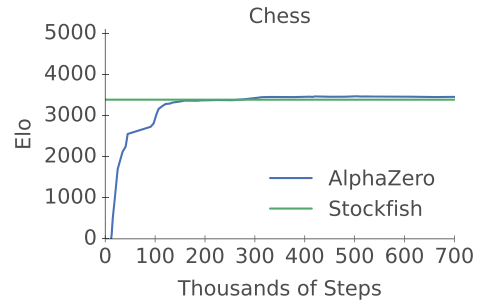
\includegraphics[width=0.6\textwidth]{figures/alpha-zero-elo-evolution.png}
    \caption{AlphaZero Elo evolution over training steps \cite{silver2018general}}
    \label{fig:alphaZeroEloEvolution}
\end{figure}

\section{Leela Chess Zero}
\label{sec:ch3sec5}

Leela Chess Zero (LCZero) is a computer chess engine based on the principles of DeepMind's AlphaZero. Since AlphaZero is not open-source, and there was no way to test the results stated in DeepMind's paper, LCZero was created by a group of developers led by Gary Linscott, who started the project in 2018. The engine was largely driven by the community of chess enthusiasts and programmers, who contributed to the project by providing computing resources.

LCZero developers also brought some key improvements to the AlphaZero approach:
\begin{itemize}
    \item Efficient implementation: LCZero is designed to run efficiently on standard hardware, such as CPUs and GPUs commonly available to consumers. This makes it more accessible than AlphaZero, which was trained on specialized hardware
    \item Improved neural network architecture: LCZero's neural network architecture is optimized for the game of chess, with modifications that allow it to better represent the game state and learn from self-play. This has led to better performance in practice. The developers also added Squeeze and Excitation (SE) layers to the neural network, which improve the representation of CNNs (Convolutional Neural Networks), by enabling them to selectively attend to the most important features of the input data
    \item Dynamic evaluation: LCZero uses a dynamic evaluation function during self-play, which allows it to better evaluate the value of positions and guide its search. Unlike AlphaZero, which uses a fixed evaluation function throughout the self-play process, LCZero updates its evaluation function after each game played, based on the results and the positions encountered. This allows it to adapt to changes in the playing style and strategy of its opponents
\end{itemize}

In April 2018, LCZero became the first engine to join the TCEC that used a deep neural network. At first, it didn't perform well, but by September 2018, it achieved a level of competitive performance comparable to the strongest chess engines in the world, and in 2019 and 2020 it won the competition. Since joining the TCEC, LCZero has achieved significant success, having won the competition twice, secured the second place on seven occasions, and achieved third place once.

On its official website \cite{lczero-training}, LCZero is currently rated over 3500 Elo points (fig. \ref{fig:leelaChessZeroEloEvolution}).

\begin{figure}[h]
    \centering
    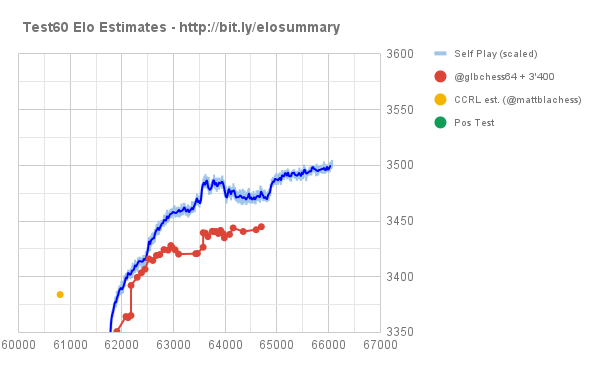
\includegraphics[width=0.9\textwidth]{figures/leela-chess-zero-elo-evolution.png}
    \caption{Leela Chess Zero Elo evolution by different metrics \cite{lczero-training}}
    \label{fig:leelaChessZeroEloEvolution}
\end{figure}
\chapter{Methodology}
\label{chap:ch4}

In this chapter I will describe the implementation of the three main steps taken by the engine to find the best move: generating legal moves for a position, searching for legally reachable positions from the current position, and then evaluating each one and determining which one is the best \cite{marsland1986review}.

% Description of the approach taken to build the chess engine
% Explanation of the AI techniques used and why they were chosen

\section{Move generation}
\label{sec:ch4sec1}

The engine computes the pseudo-legal moves of the pieces of the player that is moving, then it does each move, checks the state of the board, adds the move to the list of legal moves if the board is in a valid state, and then undoes the move.

To check the state of the board I used a threat map (fig. \ref{fig:threatMap}), which keeps track of the squares that are under attack or are defended by at least one piece (including empty squares, squares with allied pieces, and squares with opponent pieces). After each move, the threat map is updated in the following way: for each white piece on the board, it sets "IsAttackedByWhite" to true for all the squares it attacks, and for each black piece on the board, it sets "IsAttackedByBlack" to true for all the squares it attacks.

\begin{figure}
  \centering
  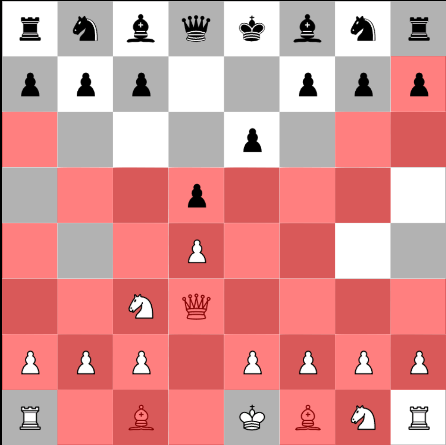
\includegraphics[scale=0.5]{figures/white-threat-map.png}
  \captionof{figure}{White threat map}
  \label{fig:threatMap}
\end{figure}

\section{Search}
\label{sec:ch4sec2}

The simplest way of searching in the game tree is through a fixed depth Minimax algorithm, which would be mathematically accurate, but would not yield good results and would be very slow. However, in combination with some optimizations and heuristics, it can compute faster and find better moves.

\subsection{Alpha-beta pruning}
\label{subsec:ch4sec2subsec1}

The Minimax algorithm was improved with Alpha-beta pruning, which preserves the accuracy of the algorithm and significantly reduces the number of nodes visited if combined with a good move ordering heuristic \cite{eric1992analysis}.

A simple pseudocode for Alpha-beta pruning is shown in fig. \ref{fig:alphabetaPseudocode}:

\begin{figure}[h]
  \centering
  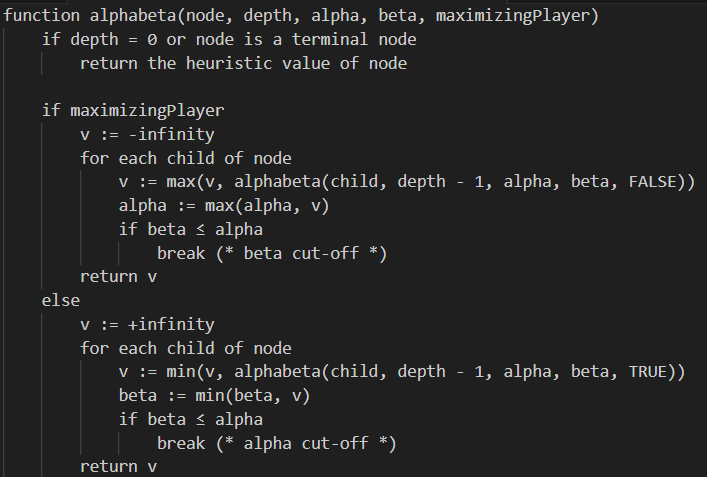
\includegraphics[scale=0.9]{figures/alphabeta-pseudocode.png}
  \captionof{figure}{Alpha-beta pruning pseudocode}
  \label{fig:alphabetaPseudocode}
\end{figure}

The heuristic I used in combination with Alpha-beta pruning is MVV-LVA (Most Valuable Victim - Least Valuable Agressor): the moves that capture pieces with high values are first, and if multiple moves capture a piece of the same value, the moves with the least valuable agressor are prioritized \cite{mvv-lva}. The heuristic is based on the observation that in chess, it is often advantageous to capture pieces of higher value than the capturing piece, while avoiding exchanges where the capturing piece is more valuable than the captured piece. It is also relatively easy to implement, and does not require much computational overhead. Other heuristics, use the evaluations of previous searches or the results from other branches, and require maintaining and updating additional data structures to keep track of the move history and their performance.

\subsection{Quiescence search}
\label{subsec:ch4sec2subsec2}

When the Minimax search reaches the maximum depth in a branch, it evaluates the position and propagates it back. With the quiescence search optimization, the position is first checked for potential moves that could disrupt the evaluation in the following move.

I considered captures and promotions to be disruptive moves, since they have a big impact on material. If there are no such moves available, the algorithm continues as normal. But if there are, the current static evaluation is kept as a "stand-pat" score (the term is used in poker, to describe a situation where a player chooses to keep their hand as it is without drawing any additional cards), to establish a lower bound on the evaluation.

The "disruptive" moves are played, and, from the positions reached, quiescence search is applied again, until a certain depth is reached. Each new position is evaluated using the static function, and if the evaluation is better than alpha (the lower bound, which is initialized with the stand-pat score), then the evaluation score is assigned to alpha. At the end of the quiescence search, the alpha score is returned. I used 4 as the maximum quiescence search depth, to allow the engine to detect certain series of exchanges, but not search too deep and use up too much time.

The stand-pat score is used based on the Null Move Observation, which states
that there is almost always a move that improves the current position - it assumes the player to move is not in Zugzwang (a position in which it is disadvantageous to move, as every move inevitably results in a worse position). The stand-pat assumes that even if all the disruptive moves are searched, and none of them increase alpha, one of the non-disruptive moves can most likely raise alpha. This is not valid if every move is searched.

\subsection{Iterative deepening}
\label{subsec:ch4sec2subsec3}

The iterative deepening starts computing the evaluations for the Minimax with depth 1, and then increments the depth up to the given maximum depth. After the time given as an input elapses, the search is stopped and the move with the best evaluation found on the previous depth search is returned. I set the maximum time to 50 seconds, but this can be easily changed from a parameter, depending on the length of the match and accuracy of moves the user of the engine desires.

\section{Evaluation}
\label{sec:ch4sec3}

I used two methods of evaluating a chess board position. The first one is a simple evaluation function based on the position of the pieces on the board, and the second one is a neural network model, trained on matches played at grandmaster level.

\subsection{Board pieces}
\label{subsec:ch4sec3subsec1}

This evaluation function assigns a value to the board configuration based on the position of the pieces and the state of the game (opening/middlegame/endgame). I considered the state to be the opening if there were less than 13 moves made, middlegame if there are at least a queen or 3 minor pieces (rook/bishop/knight) on the board, and the endgame otherwise.

\begin{figure}[h]
    \centering
    \begin{minipage}{.49\textwidth}
      \centering
      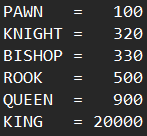
\includegraphics{figures/pieces_values.png}
      \captionof{figure}{Base values for the pieces}
      \label{fig:piecesValues}
    \end{minipage}
    \begin{minipage}{.49\textwidth}
      \centering
      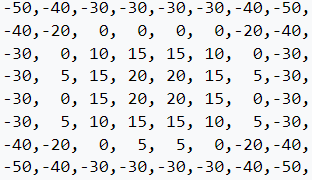
\includegraphics{figures/knight_value_table.png}
      \captionof{figure}{Knight value table}
      \label{fig:knightValueTable}
    \end{minipage}
\end{figure}

\begin{figure}[h]
    \centering
    \caption{King value tables}
    \begin{subfigure}{0.49\textwidth}
        \centering
        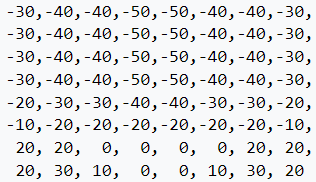
\includegraphics{figures/king_value_table_middlegame.png}
        \caption{King middlegame value table}
        \label{fig:kingValueTableMiddlegame}
    \end{subfigure}
    \begin{subfigure}{0.49\textwidth}
        \centering
        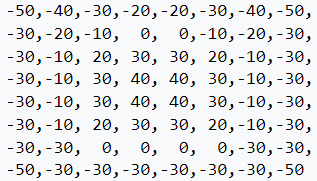
\includegraphics{figures/king_value_table_endgame.png}
        \caption{King endgame value table}
        \label{fig:kingValueTableEndgame}
    \end{subfigure}
\end{figure}

Each piece has a base value (fig. \ref{fig:piecesValues}), to which another value is added based on the square the piece occupies. Each piece has an 8x8 table, with a value for each square. The tables contain values as to encourage development of the pieces (example - fig. \ref{fig:knightValueTable} shows the table for the white knights). The tables for black pieces are horizontally simetric to the ones for the white pieces. The king has an additional table for the endgame, because in the opening and middlegame it is encouraged to castle and discouraged to move far from the first rank (fig. \ref{fig:kingValueTableMiddlegame}), while in the endgame it is encouraged to go towards the center and play an active part in the game (fig. \ref{fig:kingValueTableEndgame}) \cite{wikiEval}.

\subsection{Neural network}
\label{subsec:ch4sec3subsec2}

For the second evaluation function, I trained a neural network on grandmaster chess matches.

\subsubsection{Dataset}
\label{subsec:ch4sec3subsec2subsubsec1}

The dataset consists of chess matches played at grandmaster level downloaded in PGN format from the website chessabc.com \cite{chessabc}.

A PGN (portable game notation) file contains multiple chess matches. Each match has several headers (name of player with white pieces, name of player with black pieces, event it was played at, date it was played on, result, elo of players etc.), an empty line, and then the "movetext section". The matches in a PGN file are separated by two empty lines. Following is a sample PGN match:
\begin{figure}[h]
    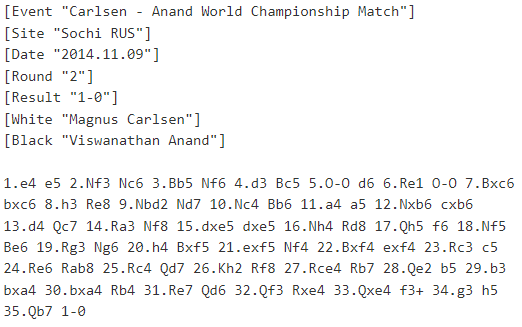
\includegraphics[width=0.8\textwidth]{figures/carlsen-anand-match.png}
\end{figure}

The movetext section contains the chess moves, move numbers, optional annotations and a concluding game termination marker (the result of the match). The result can be "1-0" (white won), "0-1" (black won) or "1/2-1/2" (draw). The moves are written in SAN (standard algebraic notation). SAN identifies each square on the board as a combination of file (a-h) and rank (1-8) (see fig. \ref{fig:boardSquares}).

\begin{figure}[h]
    \centering
    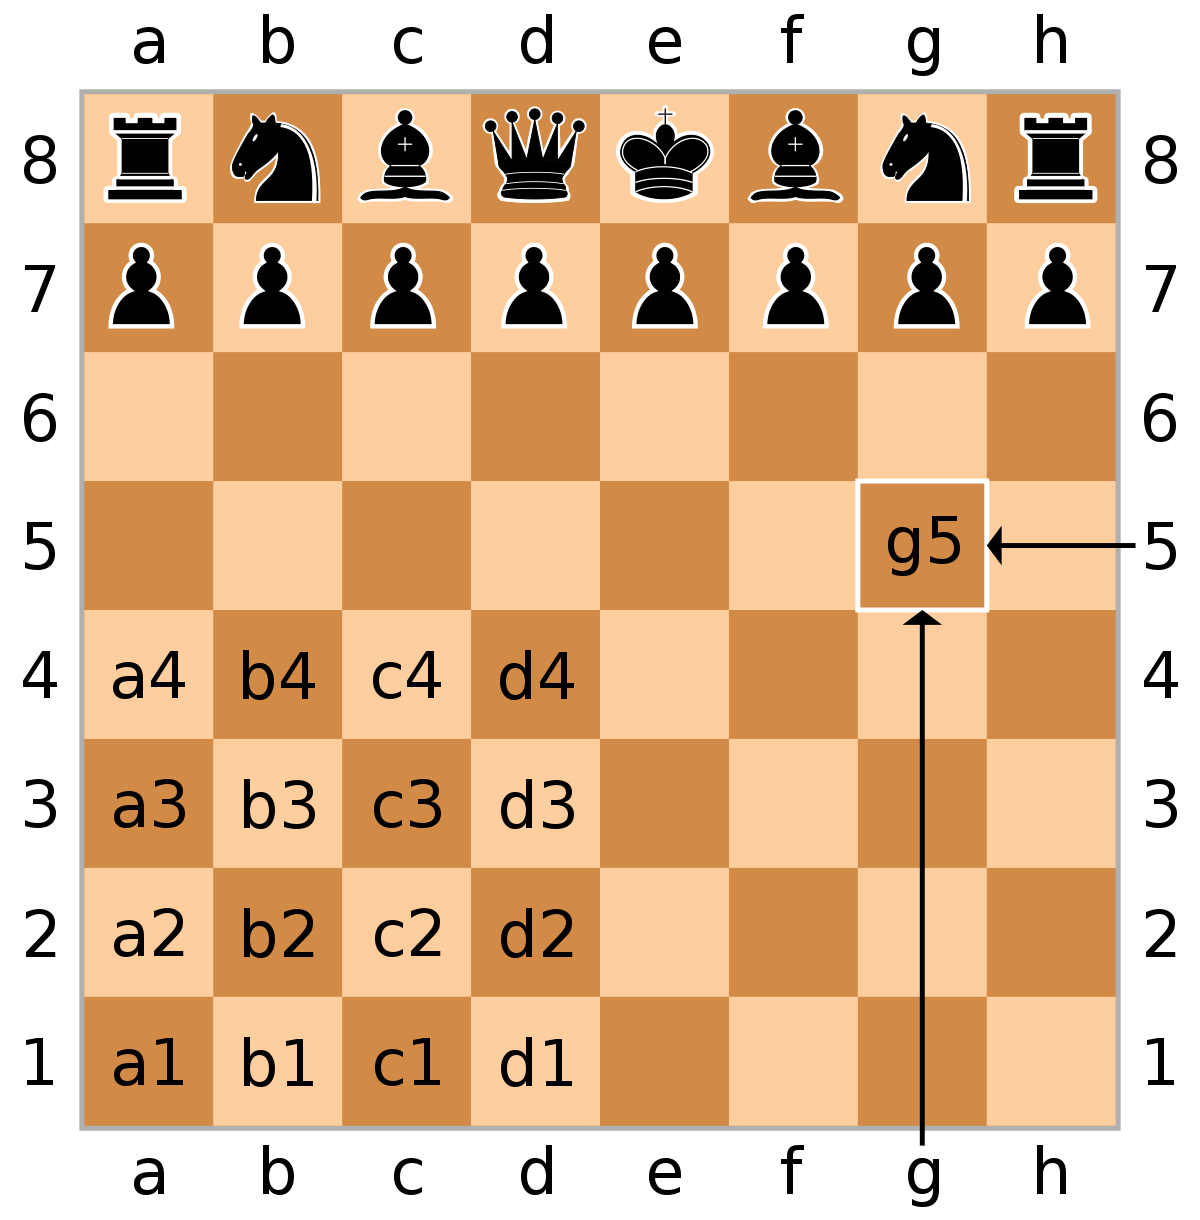
\includegraphics[width=0.4\textwidth]{figures/board-squares.png}
    \caption{Board squares}
    \label{fig:boardSquares}
\end{figure}

Each piece can be identified by a letter (K - king, Q - queen, R - rook, B - bishop, N - knight, P - pawn). Simple SAN moves contain only the destination square, and the letter of piece that moves, if the piece is not a pawn (for example, pawn to c6 is written simply as c6, while knight to c6 is written as Nc6). There are additional rules for moves \cite{edwards1994standard}:
\begin{itemize}
    \item Moves that capture a piece contain the 'x' character right before the destination square (ex: Bxb4)
    \item Castling kingside is written as 'O-O', while queenside castling is written as 'O-O-O'
    \item Moves of pawns to the last rank (promotion moves) contain the equal sign ('=') right after the destination square, followed by the letter of the piece that the pawn promotes to (ex: e8=Q)
    \item If there are multiple pieces of the same type that can move to the destination square, the file of the originating square is added right after the piece (ex: Nbc6); if this does not solve the ambiguation, the rank of the originating square is added instead (ex: N8c6), and if neither of these works, both the file and the rank are added (ex: Nb8c6)
    \item If the move checks the opponent's king, a plus sign ('+') is added at the end of the move (ex: Qe7+); if the move checkmates the opponent's king, the octothorpe sign ('\#') is added instead (ex: Qe7\#)
\end{itemize}

I computed the positions that occured in the matches in the dataset, and the value I assigned to each position is the mean of the results of the matches in which the position appeared. For example: if a certain position appeared in 10 matches, and 4 of the matches ended in a win for white, 2 in a win for black, and the other 4 were draws, the value assigned to the position is: \[\frac{(4*1)+(2*-1)+(4*0)}{10}=0.2\] (a win for white is assigned 1, a win for black is assigned -1, and a draw is 0).

% Number of positions: 8493798, number of distinct positions: 5586478

There are a number of 8.5 million positions in the dataset, and 5.5 million of those positions are distinct.

\subsubsection{Model}
\label{subsec:ch4sec3subsec2subsubsec2}

The model receives as input a position and outputs a value between -1 (winning for black) and 1 (winning for white). The position is encoded as 70 values. Following is the encoding for the starting position:

$4,1,0,0,0,0,7,10,2,1,0,0,0,0,7,8,3,1,0,0,0,0,7,9,5,1,0,0,0,0,7,11,6,1,0,$

$0,0,0,7,12,3,1,0,0,0,0,7,9,2,1,0,0,0,0,7,8,4,1,0,0,0,0,7,10,1,1,1,1,-1,0$

The input layer contains 70 nodes. The first 64 values describe the positions of the pieces (first 8 values are the pieces on a1, a2, a3, ..., a8, then b1, b2, b3, ..., b8, etc.) - each square is assigned a value based on the piece it contains (see fig. \ref{fig:squaresEncodedValues}). The next 4 values are boolean (0 - false, 1 - true) and encode the castling rights (white can castle kingside, white can castle queenside, black can castle kingside, and black can castle queenside). The next value is the en passant file (the file of the moved pawn, encoded from 0 to 7, if the last move pushed a pawn two squares, -1 otherwise). The last value is the player to move (0 for white, 1 for black).

\begin{figure}[h]
    \centering
    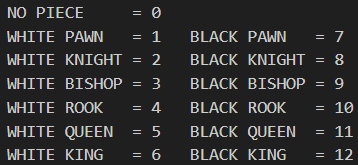
\includegraphics[width=0.6\textwidth]{figures/squares-encoded-values.png}
    \caption{Squares encoded values}
    \label{fig:squaresEncodedValues}
\end{figure}

There is only one hidden layer, with 32 nodes, with a Rectified Linear Unit (ReLU) activation function.

The output layer contains one node, the evaluation of the position, with a hyperbolic tangent (Tanh) activation function, so the output is between -1 and 1.

\subsubsection{Training}
\label{subsec:ch4sec3subsec2subsubsec3}

% 100 epoci, batch-size 64

The model was trained for 100 epochs, on a batch-size of 64, using Stochastic Gradient Descent (SGD) as an optimizer and Mean Squared Error (MSE) as a loss function.
\chapter{Technologies}
\label{chap:ch5}

\section{Technologies}
\label{sec:ch5sec1}

% Details of the programming languages, libraries, and tools used

\subsection{Chess game}
\label{subsec:ch5sec1subsec1}

% Description of tools used in building the chess game - Unity, C\#

\subsection{Chess engine}
\label{subsec:ch5sec1subsec2}

% Description of tools used in building the chess engine - C\#, keras

\chapter{Conclusions}
%\chapter*{Conclusions}
\label{conclusions}

Summary of the main findings and contributions of the thesis\\
Discussion of potential future improvements to the chess engine

%\addcontentsline{toc}{chapter}{Concluzii}
%\addcontentsline{toc}{chapter}{Conclusions}

\bibliography{references}

\end{document}
